\documentclass[letterpaper,11pt]{report}
% Change margins to 1 inch on all sides
\addtolength{\oddsidemargin}{-.875in}
\addtolength{\evensidemargin}{-.875in}
\addtolength{\textwidth}{1.75in}
\addtolength{\topmargin}{-.875in}
\addtolength{\textheight}{1.75in}
\usepackage{float}
\usepackage{graphicx}
\usepackage{footnote}
\usepackage{longtable}
\usepackage{multirow}
\usepackage{tablefootnote}
\usepackage{tabularx}
\usepackage{url}
\DeclareGraphicsExtensions{.pdf,.png,.jpg}

%%%%%%%%%%Start of report
\begin{document} 
\begin{savenotes}
\pagestyle{plain}
\title{CS896 Introduction to Web Science\\Fall 2013\\Report for Assignment 5}
\author{Corren G. McCoy}
 
\date{October 17, 2013}
\maketitle

\renewcommand*\thesection{\arabic{section}}
\setcounter{section}{0}

\setcounter{tocdepth}{4}
\tableofcontents
 \listoffigures
\newpage


%%%%%%%%%%Chapter Exercises
\section{Question 1}
\subsection{Problem}The ``friendship paradox'' (\url{http://en.wikipedia.org/wiki/Friendship_paradox}) says that your friends have more friends than you do. Determine if the friendship paradox holds for your Facebook account.  Create a graph of the number of friends (y-axis) and the friends sorted by number of friends (x-axis).  (The friends don't need to be labeled on the x-axis.)  Do include yourself in the graph and label yourself accordingly. Compute the mean, standard deviation, and median of the number of friends that your friends have.
\subsection{Response}For this problem, we used the XML file associated with Dr. Nelson's Facebook account. The file was saved in the graphML format. The social network data of interest was found in the \emph{node} tag as shown in the snippet below. We used Python to parse the XML to locate all of the \emph{node} tags. For each node, we then queried each of the enclosed \emph{data} tags until we located one with an attribute of ``friend\_count.'' If successful, we extracted the value of friend\_count from the character data (i.e., CDATA) of the tag. If the attribute was not present, the friend\_count for that particular \emph{node} was set to zero rather than excluding the \emph{node}. This was done so we could correctly determine the number of friends associated with the owner of the account. The source code for the XML parser is shown in Appendix \ref{chap:paradox}. 

\begin{verbatim}
<node id="Simeon_Warner_428351">
    <data key="Label">Simeon Warner</data>
    <data key="uid"><![CDATA[428351]]></data>
    <data key="name"><![CDATA[Simeon Warner]]></data>
    <data key="mutual_friend_count"><![CDATA[13]]></data>
    <data key="friend_count"><![CDATA[244]]></data>
</node>
\end{verbatim}

\paragraph{}To facilitate a graphical analysis, the output from the parser was saved to text file (i.e., paradox.txt) consisting of a sequential ID number and the numeric friend count. To analyze the network, we created a function in ``R'' which performed the following tasks:
\begin{itemize}
\item Accept a parameter to determine the data set to represent on the graph;
\item Read the network data from the text file created by the XML parser;
\item Sort the data by number of friends, in increasing order;
\item Calculate the mean, median, and standard deviation of the data set; and
\item Draw and annotate the resulting graph.
\end{itemize}
\paragraph{}The source code for the ``R'' function is shown in Appendix \ref{chap:p}. From the graph shown in Figure \ref{fig:facebookParadox}, we can see that the ``friendship paradox'' holds for the Facebook account. For this particular network, the owner has 165 friends, denoted by the purple marker, which is fewer than the median or typical number of 244 Facebook friends denoted by the red marker. This observation is supported by Feld's \cite{feld1991your} theory that ``friends are likely to be friendlier than average'' and therefore have a higher tendency to make more friends. We must also consider how the friendship counts at the higher end of spectrum (i.e., outliers) affect the calculation of the median value. These friends, in effect, contribute more heavily to the calculation which skews the median away from the friend count of any one individual. We are the using the median as the comparative value because the data is not symmetrical around the mean. The median, therefore, provides a way to estimate the exact midpoint of all the data.


\begin{figure}[htbp]
	\centering
		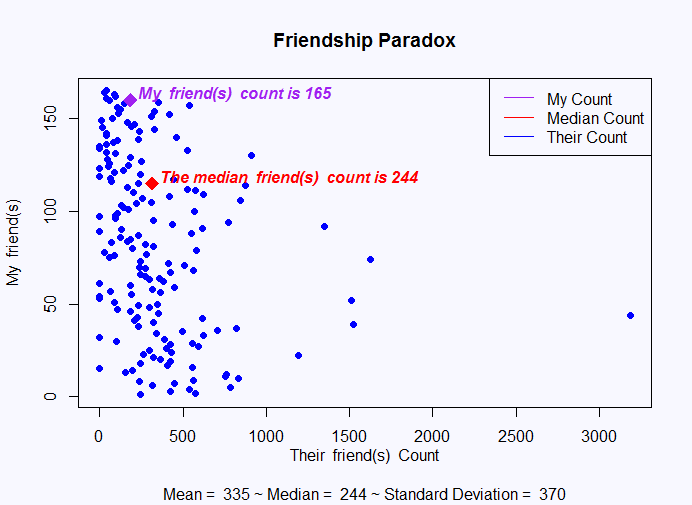
\includegraphics[width=0.80\textwidth]{facebookParadox.png}
	\caption{Friendship Paradox - Facebook}
	\label{fig:facebookParadox}
\end{figure}

%%%%%%%%%%Chapter Exercises
\section{Question 2}
\subsection{Problem}Determine if the friendship paradox holds for your Twitter account. Since Twitter is a directed graph, use ``followers''as value you measure (i.e., ``do your followers have more followers than you?''). Generate the same graph as in question \#1, and calculate the same mean, standard deviation, and median values.
\subsection{Response}For this problem, we used Dr. Nelson's Twitter account (i.e., @phonedude\_mln). His profile summary, shown in Figure \ref{fig:phonedude}, provides verification of our results as of the date we performed our calculations. We used Python to access the Twitter API, GET followers/list\footnote{\url{https://dev.twitter.com/docs/api/1.1/get/followers/list}}, which returns information about the specified user. The user object returned by the API includes a \emph{followers\_count} which indicates ``the number of followers this account currently has.'' The Tweepy Python package \footnote{\url{http://code.google.com/p/tweepy/}} provides a wrapper for all of the Twitter API methods. We used the constructs in Tweepy to traverse the list of followers and subsequently retrieve each of their followers\_count data. The source code for Python is shown in Appendix \ref{chap:getFollowers}. The output from Twitter was saved to text file (i.e., followersFile.txt) consisting of a sequential ID number, the numeric followers\_count, and the user\_name. The user\_name was included so we could search Twitter to verify the results for a particular user.

\paragraph{}For graphical analysis, we used the same ``R'' function, Appendix \ref{chap:p}, to produce the graph shown in Figure \ref{fig:followerParadox}. For re-usability of code, each data file used by the ``R'' function minimally contained an \emph{ID} and \emph{count} field.  The ``friendship paradox'' does not hold for Twitter followers. The 204 followers of @phonedude\_mln is slightly above the median of 192 for each of his followers. However, the very large value of 1,261 for the standard deviation clearly indicates a significant amount of dispersion in the data set. The wide swing in the standard deviation is most likely due to the outliers who have in the range of 9,000 to more than 10,000 followers. These outliers include @albakhakh with 9,385 followers, @bfluzin with 10,040 followers and @klischk with 10,128 followers.

\begin{figure}[htbp]
	\centering
		\includegraphics[width=0.80\textwidth]{phonedudeProfileSummary.png}
	\caption{Dr. Nelson's Twitter Profile Summary}
	\label{fig:phonedude}
\end{figure}

\begin{figure}[htbp]
	\centering
		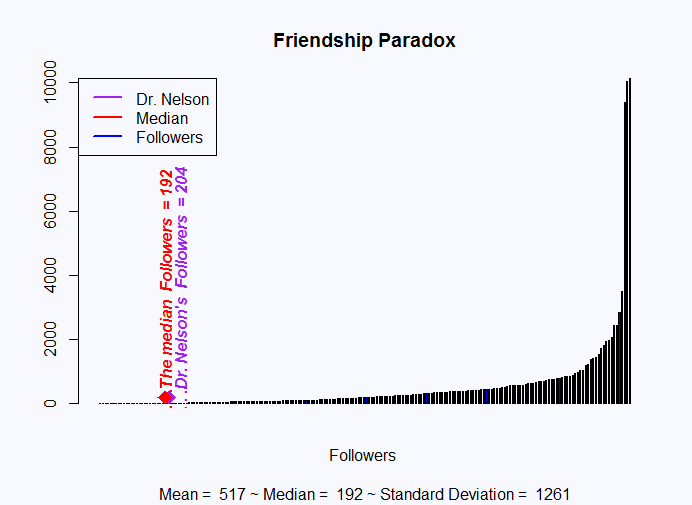
\includegraphics[width=0.80\textwidth]{followersParadox.png}
	\caption{Friendship Paradox - Followers on Twitter}
	\label{fig:followerParadox}
\end{figure}

%%%%%%%%%%Chapter Exercises
\section{Question 3 Extra Credit}
\subsection{Problem}Repeat question \#1, but with your LinkedIn profile.
\subsection{Response}Not attempted.

%%%%%%%%%%Chapter Exercises
\section{Question 4 Extra Credit}
\subsection{Problem}Repeat question \#2, but change ``followers'' to ``following''. In other words, are the people I am following following more people?
\subsection{Response}We used the same processing as noted for question 2, except instead of extracting the followers\_counts, we extracted the friends\_ count instead. The Twitter API indicates that friends\_count represents ``the number of users this account is following (AKA their ``followings'').''  The Python source code is shown in Appendix \ref{chap:getFriends}. Once again, we saved the output from Twitter to a text file (i.e., friendsFile.txt) consisting of a sequential ID number, the numerical friends\_count, and the user\_name for verification.

\paragraph{} For graphical analysis, we used the same ``R'' function, Appendix \ref{chap:p}, to produce the graph shown in Figure \ref{fig:followingParadox}. The ``friendship paradox'' holds for the users @phonedude\_mln is following. The number of people he is following consists of 73 users which is well below the median of 199 users for those he is following. This data set also has a large standard deviation of 456 which demonstrates the wide range of data points. The extreme outlier, in this case, is @smalljones who is following 3,341 users.

\begin{figure}[htbp]
	\centering
		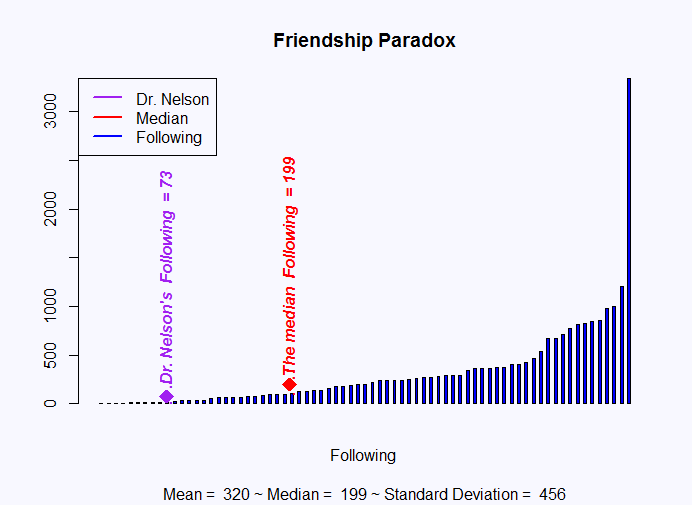
\includegraphics[width=0.80\textwidth]{followingParadox.png}
	\caption{Friendship Paradox - Following on Twitter}
	\label{fig:followingParadox}
\end{figure}

\end{savenotes}

% produce the bibliography for the citations in your paper.
\bibliographystyle{abbrv}
\bibliography{cmccoy}

\appendix
\addcontentsline{toc}{chapter}{Appendices}

%%Appendix A
\chapter{Python Source - paradox.py} \label{chap:paradox}
\input{paradox.py}
\chapter{Python Source - getFollowers.py} \label{chap:getFollowers}
\input{getFollowers.py}
\chapter{Python Source - getFriends.py} \label{chap:getFriends}
\input{getFriends.py}

\chapter{R Source - paradox.r} \label{chap:p}
\input{paradox.r}



\end{document} 
%%%%%%%%%%Ed of report
